\subsubsection{First Measurements}





\begin{figure}
\centering
\subcaptionbox{
Scatter plot of $10000$ IQ-records with an alpha value of $0.1$ while the JPC is turned off.
\label{fig:IQ:first_measurements:IQ_jpc_off}}
[8.6cm]{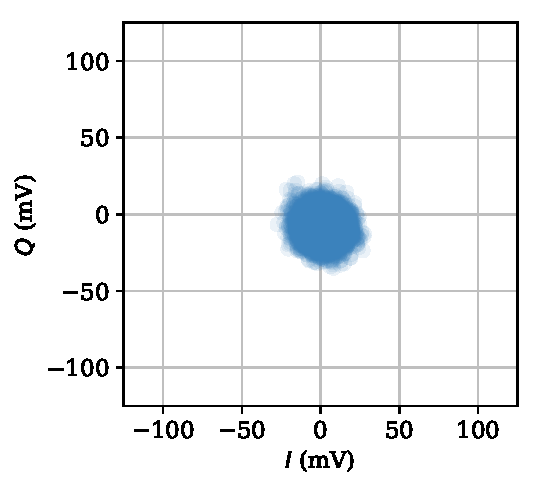
\includegraphics[width=8.6cm]{plots/IQ_plots/first_measurements/IQ_jpc_off.pdf}}
~
\subcaptionbox{
Transmission spectra of the cavity measured with a VNA while the JPC is turned off (orange) and on (blue). The JPC is operated with a gain of $\SI{27}{dB}$ at the IQ-readout frequency (dashed black line).
\label{fig:IQ:first_measurements:JPC_curves}}
[8.6cm]{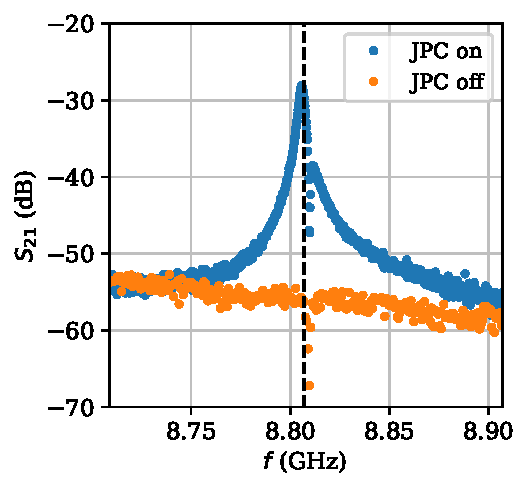
\includegraphics[width=8.6cm]{plots/IQ_plots/first_measurements/vna_jpc_on_off.pdf}}
~
\subcaptionbox{
Same measurement as in (\subref{fig:IQ:first_measurements:IQ_jpc_off}) with JPC turned on. The improvement in SNR clearly resolved three distinct features.
\label{fig:IQ:first_measurements:IQ_jpc_on}}
[8.6cm]{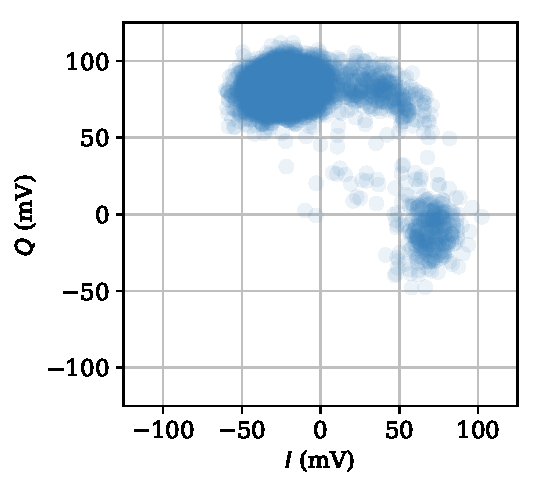
\includegraphics[width=8.6cm]{plots/IQ_plots/first_measurements/IQ_jpc_on.pdf}}
\caption{
First IQ-measurements with $T_{mes} = \SI{640}{ns}$ at $P_{mes} = \SI{16}{dBm}$ and a probe frequency $f_{P} = \SI{8.8069}{GHz}$. Without the JPC the cahracteristic features, that would indicate the quantum state of the system, remain hidden in the noise (\subref{fig:IQ:first_measurements:IQ_jpc_off}). Turning on the JPC with the maximum gain frequency tuned to the IQ readout frequency $f_{P}$ (\subref{fig:IQ:first_measurements:JPC_curves}) increases the SNR and reveals three distinct spots at which the individual measurement records accumulate (\subref{fig:IQ:first_measurements:IQ_jpc_on}). Their distribution clearly deviate from the expected gaussian shape. This is due to the high readout-power and hard driving of the JPC.}
\label{fig:IQ:first_measurements:main}
\end{figure}
